\documentclass[10pt,twocolumn]{article}
\usepackage[margin=0.7in]{geometry}
\usepackage[T1]{fontenc}
\usepackage{lmodern}
\usepackage{microtype}
\usepackage{booktabs}
\usepackage{tabularx}
\usepackage{amsmath,amssymb}
\usepackage{graphicx}
\usepackage{xcolor}
\usepackage{tikz}
\usetikzlibrary{positioning,arrows.meta,calc}
\usepackage{enumitem}
\usepackage{url}
\usepackage[hidelinks]{hyperref}
\usepackage{cleveref}
\graphicspath{{../paper/}}
\setlist{nosep,leftmargin=*}
\setlength{\textfloatsep}{8pt plus 2pt minus 2pt}
\setlength{\floatsep}{6pt plus 2pt minus 2pt}

\title{\vspace{-8mm}Prove Less, Repair Better --- Mid-Submission Progress Report\\[2pt]
\large Automation-Friendly Program Repair for Small Models in Lean~4\vspace{-1mm}}
\author{Agents of Ultron: Inesh Dheer (2023111010) \and Poojitha J (2024101088) \and Gracy Garg (2023101118)\\
\small Agentic Software Engineering (CS6.403), IIIT Hyderabad \quad
Repository: \url{https://github.com/amoiba42/Leanstein}}
\date{6 November 2026\vspace{-4mm}}

\begin{document}
\maketitle

\section*{Summary}
We proposed testing whether small, locally runnable models produce more \emph{verified} program repairs in
Lean~4 when they repair only the code and leave the proof to a fixed, pre-registered portfolio of Lean automation
(condition C), rather than writing proofs themselves (B). By this milestone the project has gone well past a
prototype. The harness is complete and tested; we built a buggy-VERINA dataset with hidden tests; we ran a pilot and
a power analysis; we froze the configuration; and we ran the \textbf{full pre-registered study (12,249 runs)} and
its analysis, all on one 48\,GB MIG slice of an NVIDIA RTX PRO 6000 Blackwell. The main result supports the
hypothesis: C beats B for both primary models ($p_\text{Holm}<0.001$). Against a proof-writing agent that gets the
same automation first (BP), C is level or slightly better, and cheaper. The remaining work is an energy calibration
study, human confirmation of the audit, and polishing the paper.

\section{What has been built}
\textbf{Harness (\texttt{prl/}, 5.4k lines of Python; 96 unit and 24 Lean integration tests, all passing).}
\begin{itemize}
\item \emph{Tasks} (\texttt{prl/tasks}): loads VERINA at a pinned commit, splits each task into locked regions
(specification, theorem statement, tests) and editable ones (code, helpers, proof), and checks eligibility.
\item \emph{Bugs} (\texttt{prl/natural}, \texttt{prl/mutate}): \emph{natural} bugs are zero-shot implementations by
Qwen3.5-0.8B/9B that compile and fail a test; \emph{mutants} come from 8 operators (arithmetic, relational, boolean,
constant, condition negation, branch swap, off-by-one, argument swap).
\item \emph{Hidden tests} (\texttt{prl/testgen}): 30 generated inputs per family whose precondition is \emph{proved
in Lean}, with expected outputs from the reference. They are never shown to a model.
\item \emph{Verification} (\texttt{prl/lean}): a persistent Lean~4.24 + Mathlib server per worker; static
integrity checks (no \texttt{sorry}, axioms, \texttt{native\_decide}, locked-name redefinitions, or proof text in
code-only conditions); an axiom check; and a frozen two-tier tactic portfolio (Tier~L: \texttt{decide},
\texttt{simp}, \texttt{simp\_all}, \texttt{omega}, \texttt{split}; Tier~H: \texttt{grind}, \texttt{aesop},
induction templates).
\item \emph{Conditions and driver} (\texttt{prl/conditions}, \texttt{prl/driver}): conditions A, B, BP, C,
C-plain, S, S-plain, Bhammer and T behind one interface, with matched budgets (8 generations, 48k tokens, 600\,s
of inference). Infrastructure failures are retried without charging the model, and every attempt is logged with
its tokens, model time and Lean time.
\item \emph{Analysis} (\texttt{prl/analysis}): family-level paired sign-flip tests with Holm correction, cluster
bootstrap, power simulation, shaping-vs-reverting classification, code-shape features, B$\to$C
cross-evaluation, and the audit sampler.
\item \emph{Pre-registration} (\texttt{prereg/}): study parameters, portfolio, prompts and power note, hashed by
\texttt{prl freeze}. The driver refuses confirmatory runs on any mismatch, and changes go to
\texttt{prereg/deviations.md}.
\end{itemize}
\Cref{fig:pipeline} shows the architecture. Design documents (requirements, HLD, LLD, architecture decisions,
implementation plan) are in \texttt{docs/}, and the run record is in \texttt{context/IREL\_RUNS.md}.

% Method overview: from a VERINA task to a verdict. Fixed coordinates so no edge crosses a box.
\begin{figure*}[t]
\centering
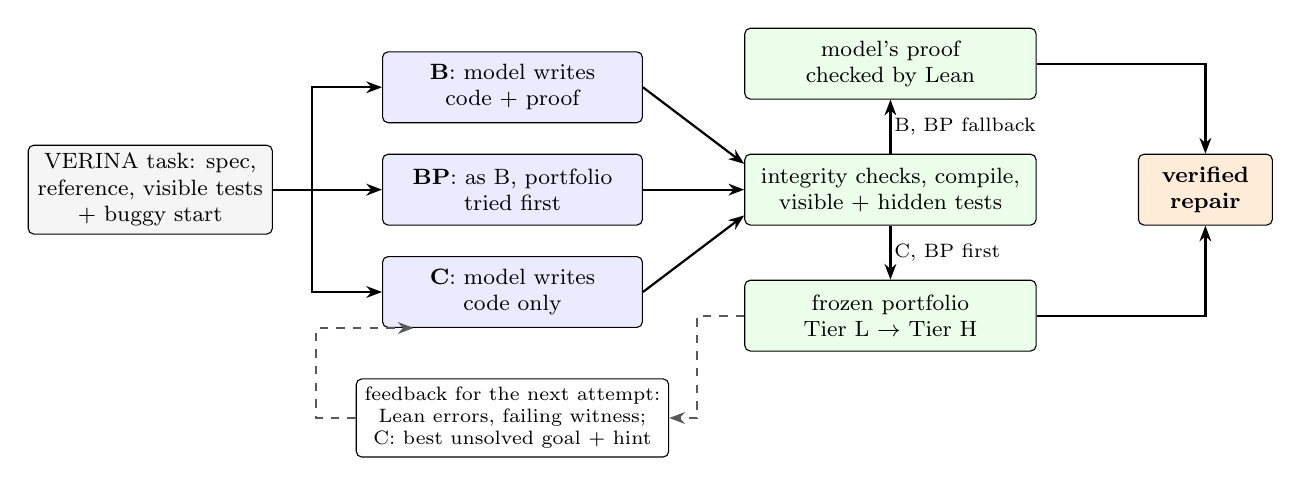
\begin{tikzpicture}[
  box/.style={draw, rounded corners=2pt, align=center, font=\footnotesize, minimum height=9mm, inner sep=3pt},
  data/.style={box, fill=gray!8, minimum width=31mm},
  model/.style={box, fill=blue!8, minimum width=33mm},
  lean/.style={box, fill=green!8, minimum width=37mm},
  verdict/.style={box, fill=orange!15, font=\footnotesize\bfseries, minimum width=17mm},
  arr/.style={-{Stealth[length=2mm]}, thick},
  fb/.style={-{Stealth[length=2mm]}, thick, dashed, gray!70!black},
  lab/.style={font=\scriptsize, fill=white, inner sep=1pt}]
\node[data]    (in)     at (0, 0)      {VERINA task: spec,\\reference, visible tests\\+ buggy start};
\node[model]   (B)      at (4.6, 1.3)  {\textbf{B}: model writes\\code + proof};
\node[model]   (BP)     at (4.6, 0)    {\textbf{BP}: as B, portfolio\\tried first};
\node[model]   (C)      at (4.6, -1.3) {\textbf{C}: model writes\\code only};
\node[lean]    (gate)   at (9.4, 0)    {integrity checks, compile,\\visible + hidden tests};
\node[lean]    (mp)     at (9.4, 1.6)  {model's proof\\checked by Lean};
\node[lean]    (port)   at (9.4, -1.6) {frozen portfolio\\Tier L $\to$ Tier H};
\node[verdict] (ok)     at (13.4, 0)   {verified\\repair};
\node[box, font=\scriptsize, minimum width=33mm] (fbk) at (4.6, -2.9)
  {feedback for the next attempt:\\Lean errors, failing witness;\\C: best unsolved goal + hint};
\draw[arr] (in.east) -- ++(0.5,0) |- (B.west);
\draw[arr] (in.east) -- (BP.west);
\draw[arr] (in.east) -- ++(0.5,0) |- (C.west);
\draw[arr] (B.east) -- (gate.170);
\draw[arr] (BP.east) -- (gate.west);
\draw[arr] (C.east) -- (gate.190);
\draw[arr] (gate.north) -- node[lab, right]{B, BP fallback} (mp.south);
\draw[arr] (gate.south) -- node[lab, right]{C, BP first} (port.north);
\draw[arr] (mp.east) -| (ok.north);
\draw[arr] (port.east) -| (ok.south);
\draw[fb] (port.west) -- ++(-0.6,0) |- (fbk.east);
\draw[fb] (fbk.west) -- ++(-0.5,0) |- (C.200);
\end{tikzpicture}
\caption{Method. Every condition gets the same buggy start, the same visible information and the same budget
(8 generations, 48k tokens, 600\,s of inference). A candidate must pass integrity checks, compile and pass every
visible and hidden test before any proof is tried; hidden tests are never shown to the model. In B the model's own proof must check; in C the model writes
no proof and a frozen two-tier portfolio of Lean automation must prove the unchanged specification; BP tries the
portfolio first and falls back to the model's proof. A failed attempt returns feedback for the next one (dashed),
in every condition except the single-shot baseline A.}
\label{fig:pipeline}
\end{figure*}


\textbf{Dataset.} 189 VERINA tasks were screened and 184 are eligible (104 basic, 80 advanced). They are split by
family into pilot (20), main (114) and held-out (50). Natural bugs cover 33 \texttt{main} families. Because that
is below the pre-registered 60, the fallback pool (natural $\cup$ mutant, 106 families) applies. The portfolio alone
proves 22.3\% of eligible references (basic 35.6\%, advanced 5.0\%); the screening gate needed $\geq$20\%.

\section{Demonstration on a representative task}
\texttt{verina\_basic\_1} asks whether two integers have opposite signs. Its postcondition is
$((a<0\wedge b>0)\vee(a>0\wedge b<0)) \leftrightarrow \mathit{result}$. The natural bug (from Qwen3.5-9B) returns
\texttt{true} for $a=0,b=-10$:
\begin{quote}\small\ttfamily if a < 0 then if b > 0 then true else false\\ else if b < 0 then true else false\end{quote}
\textbf{B (Qwen3.5-4B, seed 11)} fixes the code on its second attempt
(\texttt{(a < 0 $\wedge$ b > 0) $\vee$ (a > 0 $\wedge$ b < 0)}). It then spends all remaining attempts on
proofs that begin with \texttt{intro}, which Lean rejects every time (``no additional binders''), and ends
unresolved with correct code. \textbf{C} submits the same code on its \emph{first} attempt. It passes all visible
and hidden tests, the portfolio's first Tier-L entry (\texttt{simp}) proves it, and the run ends as a verified
repair. This pattern is common: when B's code compiled but its proof failed, C's pipeline would have verified
31\% of those attempts (4B).

\section{Evaluation results to date}
\begin{table}[!h]\centering\small
\caption{RQ1 (confirmatory), \texttt{main} split, 106 families, family-level verified-repair rate. One-sided
sign-flip test, Holm over the four tests, 95\% family-cluster bootstrap CI.}\label{tab:rq1}
\setlength{\tabcolsep}{3pt}
\begin{tabular}{@{}llrrrr@{}}\toprule
Model & Test & C & Other & Diff.\ [95\% CI] & $p_\text{Holm}$ \\\midrule
Qwen3.5-2B & C vs B  & 27.7 & 2.2  & +25.5 [18.2, 33.0] & $<$0.001 \\
Qwen3.5-2B & C vs BP & 27.7 & 22.6 & +5.0 [1.6, 8.8]   & 0.012 \\
Qwen3.5-4B & C vs B  & 33.0 & 17.6 & +15.4 [9.4, 21.7] & $<$0.001 \\
Qwen3.5-4B & C vs BP & 33.0 & 32.7 & +0.3 [$-$2.8, 3.5] & 0.50 \\\bottomrule
\end{tabular}
\end{table}

\begin{figure*}[t]\centering
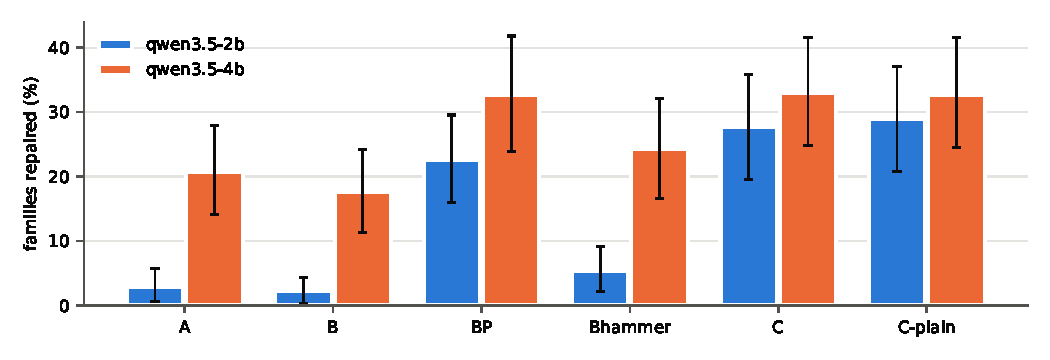
\includegraphics[width=0.82\textwidth]{fig_rates.pdf}\vspace{-2mm}
\caption{Family-level verified-repair rate per condition (\texttt{main}, primary bug pool), with 95\% bootstrap
intervals. Bhammer is exploratory.}\label{fig:rates}
\end{figure*}

\begin{table*}[!t]\centering\small
\caption{Original proposal vs.\ the study as built and run. Reasons are in \texttt{docs/final\_proposal.md} and
\texttt{prereg/deviations.md}.}\label{tab:changes}
\begin{tabularx}{\textwidth}{@{}l>{\raggedright\arraybackslash}p{0.27\textwidth}>{\raggedright\arraybackslash}X@{}}\toprule
Aspect & Original proposal & Now \\\midrule
Models & Qwen2.5-Coder 1.5B and 3B, 4-bit, 8\,GB laptop GPU & Qwen3.5-2B and 4B (primary), Gemma-4-E4B (second
family), Goedel-Code-Prover-8B (proof specialist); all 4-bit \\
Hardware & one laptop & one 48\,GB MIG slice of an RTX PRO 6000 Blackwell, used for every step from dataset to
analysis; an earlier freeze prepared on a laptop was superseded before any result was read \\
Conditions & A, B, C, optional D (progressive hints) & added BP (portfolio first, then the model's proof),
C-plain (replaces D as the feedback test), S/S-plain (re-shaping correct code), T (screening), Bhammer
(exploratory) \\
Bugs & injected defects only & natural bugs from other models as the primary pool, mutants as fallback and
stratum \\
Hidden tests & independent behavioural tests & generated inputs with Lean-\emph{proved} preconditions \\
Sampling & $k=4$ candidates per round & 2 per round in C, so total budgets match B \\
Scale & 60--100 families & 114 \texttt{main} + 50 held-out families, 3 seeds; held-out analysed once, separately \\
Rigour & pre-registered portfolio & full pre-registration with a hash freeze, pilot power simulation, Holm
correction, stop rules and a public deviation log \\
Added analyses & --- & shaping vs reverting, B\_noauto, B$\to$C cross-evaluation, code-shape catalogue,
integrity audit \\
Time cap & --- & 600\,s of inference per run; a calibration showed a 240\,s cap was not condition-neutral \\
\bottomrule
\end{tabularx}
\end{table*}

The study ran 12,249 runs from 5 Nov 21:06 to 6 Nov 11:49: \texttt{main} 6,930 (Qwen3.5-2B/4B $\times$ A, B, BP,
C, C-plain $\times$ 3 seeds), held-out 1,710, study S 1,068, Gemma 693, Goedel 462 and Bhammer 1,386. There was
1 infrastructure failure, completed on resume; no run hit the time cap and no stop rule fired.
\begin{itemize}
\item \textbf{RQ1} (\cref{tab:rq1,fig:rates}): C beats B clearly for both models. C vs BP is +5.0\,pp for 2B and a
tie for 4B, as the pre-freeze power analysis predicted (power 0.71 and 0.08). The \textbf{held-out split}
replicates C over B (+18.8 and +19.6\,pp, $p_\text{Holm}=0.001$), and C vs BP ties there for both models.
\item \textbf{RQ2, mechanism}: many C successes are \emph{shaping}, meaning the reference itself is not provable,
so the repair must change the code's shape (81 of 191 for 4B; 56 are reverts). Re-shaping \emph{correct} code
(study S) is rare and hint-independent (4B: 12.7\% in both S and S-plain).
\item \textbf{RQ3, feedback}: the structured hint does not beat a plain retry (C vs C-plain: $-$1.3 and
+0.3\,pp, n.s.).
\item \textbf{RQ4, code shapes}: recursion defeats the automation. The portfolio proves 0 of 101 recursive
references against 49\% of the rest. \texttt{match}, \texttt{a[i]!} indexing and \texttt{Nat}/\texttt{Int}
casts also hurt.
\item \textbf{RQ5, cost and scale}: for 4B, C uses 37k tokens per verified repair against 65k for BP and 165k
for B, and 68\,s of inference per run against 162\,s and 150\,s. Gemma-4-E4B shows the same pattern (C 30.2\%,
B 1.9\%, BP 27.4\%). The 8B proof specialist Goedel-Code-Prover (A and B only) verifies 16.5--20.8\% of runs,
below Qwen3.5-4B in C (27.6\%).
\item \textbf{Is B a strawman?} B stays well below C even when single-call automation proofs are not counted
(B\_noauto) and when it is told the tactics (Bhammer, 24.2\% vs C 33.0\% for 4B). The audit found no
specification gaming, and no run was verified but behaviourally wrong.
\end{itemize}

\begin{table}[!h]\centering\small
\caption{Per-run verified-repair rate (\%) by bug type, \texttt{main}, Qwen3.5-2B and 4B pooled (the original
H2). $n$ = buggy instances.}\label{tab:bugtype}
\setlength{\tabcolsep}{4pt}
\begin{tabular}{@{}lrrrrr@{}}\toprule
Bug type & $n$ & A & B & BP & C \\\midrule
arithmetic operator & 44 & 14.8 & 11.4 & 36.4 & 40.2 \\
constant & 39 & 17.5 & 15.8 & 26.5 & 35.5 \\
boolean operator & 7 & 4.8 & 0.0 & 9.5 & 26.2 \\
relational flip & 25 & 7.3 & 4.7 & 16.7 & 20.0 \\
negated condition & 57 & 3.5 & 2.6 & 19.0 & 17.3 \\
swapped branches & 16 & 1.0 & 0.0 & 14.6 & 16.7 \\
natural (model-written) & 34 & 2.9 & 0.0 & 9.8 & 15.7 \\
off-by-one / arg.\ swap & 9 & 1.9 & 5.6 & 11.1 & 7.4 \\\bottomrule
\end{tabular}
\end{table}

\textbf{By bug type} (\cref{tab:bugtype}): local operator and constant bugs benefit most, as H2 predicted.
Natural bugs are harder for every condition, but only C and BP repair them at all.

\section{Known failures and limitations}
\begin{itemize}
\item \textbf{Energy (deviation D-1).} The energy meter read the NVML counter of physical GPU 0 instead of our
slice, because NVML ignores the CUDA device mask. Its CPU estimate also mixed two concurrent jobs. No energy
figure is reported yet; the calibration study below will fill this in.
\item \textbf{Audit pending human confirmation (D-3).} We read all 333 sampled successes (0 spec-gaming, 27
correct but unnatural), but a team member still has to confirm them. The spec-copying flag fires on correct
restatements of executable postconditions, so its threshold is too low for VERINA.
\item \textbf{Statistical power.} C vs BP is underpowered by VERINA's fixed size (114 \texttt{main} families), so the
4B tie is reported as a tie, not as evidence of no difference.
\item \textbf{Coverage.} Natural bugs reach only 33 families (hence the fallback pool), and no condition repairs
any of the 10 held-out natural-bug families. The portfolio proves 5\% of advanced references and none that use
recursion.
\item \textbf{Integrity rejections} are frequent in proof-writing conditions (5.7k rejected attempts in B against
1.7k in C). Most are malformed outputs (lemmas in the helper region, duplicate definitions), not cheating.
\item \textbf{Two analysis bugs} found after the runs were fixed and logged (D-2): the audit sampler crashed on a
pandas name clash and dropped a column. Neither affects a verdict.
\item \textbf{Scope.} The models are 4-bit only, the functions are small, and everything ran on one GPU model.
\end{itemize}

\section{Changes from the original proposal}
\Cref{tab:changes} summarises the changes. They strengthen the test of the hypothesis: BP isolates ``do not
write proofs'' from ``automation exists'', and natural bugs, held-out replication and the freeze guard against
over-fitting the method to the benchmark.

\section{Milestones and remaining work}
\textbf{Achieved} (dates in 2026): repository and v2 design (2 Nov); harness and tests (2--3 Nov); review
revisions (cross-evaluation, power simulation, Bhammer; 3 Nov); the seven team decisions as ADRs and the first
freeze (4--5 Nov); a from-scratch rerun on the GPU server, with dataset, probes, a 492-run pilot, power note and
second freeze (5 Nov, 21:06); the full study, analysis and paper draft (6 Nov).
\texttt{docs/implementation\_plan.md} tracks every task.

\textbf{Repository and commits.} The repository (\url{https://github.com/amoiba42/Leanstein}) has team commits
on \texttt{main} since 2 Nov, plus review branches (\texttt{alternate}, \texttt{working}) whose
changes were merged as revision~3. In order: the initial repository and v2 design, docs and harness; the
revision-3 additions; the ADRs for the seven team decisions; the first freeze and run handover; and, with this
submission, the IREL dataset, run logs, results, paper and this report. Generated artefacts (\texttt{data/},
\texttt{runs/} without raw model outputs, \texttt{results/}) are committed as research artefacts so that every
number can be traced back to a run.

\textbf{Remaining before the final submission:}
\begin{enumerate}
\item \textbf{Energy study (RQ5).} Calibrate joules per token for each model on our slice. We will alternate
loaded and idle readings of GPU power under the study's concurrency, then multiply by the tokens each condition
used. CPU energy will come from per-run Lean seconds. These are estimates, logged as a deviation.
\item Human confirmation of the 333-run audit.
\item Annotated before/after examples for the code-shape catalogue (RQ4).
\item Paper polish and a venue choice (a workshop such as LLM4Code or FormaliSE). An optional CLEVER replication if
time allows.
\end{enumerate}
The paper draft with every result filled in is \texttt{paper/main.pdf}. All results are in \texttt{results/},
and all run logs except raw model outputs are in \texttt{runs/}.

{\small
\bibliographystyle{plain}
\begin{thebibliography}{1}\setlength{\itemsep}{0pt}
\bibitem{verina} Z.~Ye et al. VERINA: Benchmarking verifiable code generation. ICLR, 2026.
\end{thebibliography}}
\end{document}
